\documentclass{standalone}

\usepackage{tikz,pgfplots}
\usepackage{siunitx}

% Set default column separator for table (csv files)
\pgfplotsset{table/col sep=comma}

\begin{document}
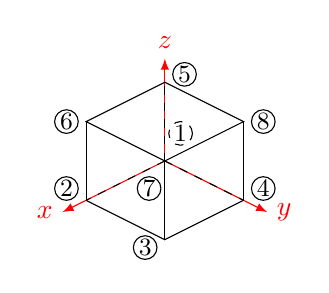
\begin{tikzpicture}[x={(-1cm,-0.5cm)}, y={(1cm,-0.5cm)}, z={(0cm,1cm)}]
% coordinate system
\coordinate (O) at (0, 0, 0);
\draw[-latex, red] (O) -- +(1.3, 0,  0) node [left] {$x$};
\draw[-latex, red] (O) -- +(0,  1.3, 0) node [right] {$y$};
\draw[-latex, red] (O) -- +(0,  0, 1.3) node [above] {$z$};
% mesh
\draw[dashed] (0,0,0) -- (1,0,0);
\draw[dashed] (0,0,0) -- (0,1,0);
\draw (1,0,0) -- (1,1,0) -- (0,1,0);
\draw (0,0,1) -- (1,0,1) -- (1,1,1) -- (0,1,1) -- cycle;
\draw[dashed] (0,0,0) -- (0,0,1);
\draw (1,0,0) -- (1,0,1);
\draw (1,1,0) -- (1,1,1);
\draw (0,1,0) -- (0,1,1);
% numbers
\draw[dashed] (-0.1,0.1,0.35) ellipse (0.15cm and 0.15cm) node {\small $1$};
\draw (1.125,-0.125,0.15) ellipse (0.15cm and 0.15cm) node {\small $2$};
\draw (1.125,0.875,-0.1) ellipse (0.15cm and 0.15cm) node {\small $3$};
\draw (-0.125,1.125,0.15) ellipse (0.15cm and 0.15cm) node {\small $4$};
\draw (-0.125,0.125,1.1) ellipse (0.15cm and 0.15cm) node {\small $5$};
\draw (1.125,-0.125,1) ellipse (0.15cm and 0.15cm) node {\small $6$};
\draw (1.1,0.9,0.65) ellipse (0.15cm and 0.15cm) node {\small $7$};
\draw (-0.125,1.125,1) ellipse (0.15cm and 0.15cm) node {\small $8$};

\end{tikzpicture}
\end{document}

